\documentclass{article}

\usepackage[utf8]{inputenc}
\usepackage[T1]{fontenc}
\usepackage{lipsum}
\usepackage{graphicx}
\usepackage{amsmath}
\usepackage[margin=1in]{geometry}
\usepackage{titlesec}
\usepackage{enumitem}
\usepackage{geometry}
\usepackage{tabularx}
\usepackage{caption}
\usepackage{fixltx2e}
\usepackage{booktabs}
\usepackage{float}  
\usepackage{graphicx}
\usepackage{floatflt,epsfig}
\usepackage[margin=1in]{geometry} 
\usepackage{lipsum}
\usepackage{graphicx}
\usepackage{listings}
\usepackage{xcolor}
\usepackage{color}

\definecolor{dkgreen}{rgb}{0,0.6,0}
\definecolor{gray}{rgb}{0.5,0.5,0.5}
\definecolor{mauve}{rgb}{0.58,0,0.82}
\lstset{language=SQL,
  basicstyle={\small\ttfamily},
  belowskip=3mm,
  breakatwhitespace=true,
  breaklines=true,
  classoffset=0,
  columns=flexible,
  commentstyle=\color{dkgreen},
  framexleftmargin=0.25em,
  frameshape={}{yy}{}{},
  keywordstyle=\color{blue},
  numbers=none,
  numberstyle=\tiny\color{gray},
  showstringspaces=false,
  stringstyle=\color{mauve},
  tabsize=3,
  xleftmargin =1em
}

\titleformat{\section}[block]
{\large\bfseries}{\thesection}{1em}{}

\titleformat{\subsection}[block]
{\normalfont\large\bfseries}{\thesubsection}{1em}{}

\begin{document}

\pagestyle{empty}

\begin{titlepage} 
\begin{center}
    {{\Large{\textsc{Alma Mater Studiorum - Università di Bologna}}}}
    \rule[0.1cm]{\textwidth}{0.1px}
    \rule[0.5cm]{\textwidth}{0.6px}\\
    {\large{SCUOLA DI SCIENZE \\ Corso di Laurea in Informatica per il Management}}
\end{center}

\vspace{50px}

\begin{center}
    {\LARGE{{\bf Piattaforma ESQL}}}\\
\end{center}

\vspace{115px}
\par
\noindent
\begin{minipage}[t]{0.04\textwidth}
~
\end{minipage}
\begin{minipage}[t]{0.4\textwidth}
\end{minipage}
\hfill
\begin{minipage}[t]{0.4\textwidth}\raggedleft
    {\fontsize{12}{13}{DOCUMENTAZIONE SVOLTA DA:}\\
\fontsize{12}{13}{\it Canghiari Matteo \\ De Rosa Davide \\ Nadifi Ossama}}
\end{minipage}
\begin{minipage}[t]{0.04\textwidth}
~
\end{minipage}

\vspace*{210px}

\begin{center}
    \large{Anno Accademico 2023/2024}
\end{center}
\end{titlepage}

\section{Analisi dei requisiti}
\setcounter{subsection}{1}
\large
All'interno di questa prima sezione, si adotta un approccio orientato ad un'analisi degli aspetti principali inerenti al progetto, mediante una serie di azioni mirate per rendere il più comprensibile possibile il documento di specifica, attraverso la scelta del corretto livello di astrazione, la standardizzazione della struttura delle frasi oppure tramite la decomposizione del testo in espressioni omogenee.

\subsection{Documento di specifica}
\large
Tutti gli utenti della piattaforma dispongono di un indirizzo email, nome, cognome e, opzionalmente, di un recapito telefonico. Gli utenti possono essere suddivisi in due categorie principali: docenti e studenti. I docenti forniscono informazioni sul dipartimento di afferenza e sul corso di cui sono titolari.
Gli studenti forniscono informazioni sull'anno di immatricolazione e un codice alfanumerico univoco.
I docenti hanno la possibilità di creare tabelle di esercizio, ognuna caratterizzata da un nome, una data di creazione e un numero di righe specificato. Le tabelle di esercizio sono correlate a un insieme di attributi, ciascuno con un nome, un tipo e la possibilità di far parte della chiave primaria della tabella di esercizio.
Inoltre, i docenti possono creare test, ciascuno con un titolo univoco, una data di creazione e la possibilità di includere una foto. Ogni test può contenere diversi quesiti, ciascuno con un numero progressivo, un livello di difficoltà, un campo descrizione e un numero di risposte. I quesiti fanno riferimento a una o più tabelle di esercizio creati dal docente.
I quesiti possono appartenere esclusivamente a due categorie: quesiti a domanda chiusa e quesiti di codice. Le domande chiuse hanno una serie di opzioni di risposta, ciascuna con una numerazione e un campo testo. I quesiti di codice hanno una o più soluzioni definite come sketch di codice.
Ogni test ha un campo booleano VisualizzaRisposte, che, se impostato su true, rende visibili le risposte dei quesiti agli studenti; altrimenti, rimangono nascoste. Gli studenti possono svolgere un test, fornendo una o più risposte per ciascun quesito. Si tiene traccia del completamento del test, ovvero la data di inserimento della prima risposta, la data di inserimento dell'ultima risposta e lo stato.
Nel caso di quesiti a domanda chiusa, la risposta consiste potenzialmente nell'insieme dell'opzioni disponibili. Nel caso di quesiti di codice, la risposta consiste in un campo testo. È prevista la possibilità per gli studenti di inviare più risposte per lo stesso quesito in istanti diversi. Ogni risposta dispone di un campo esito, un campo booleano che definisce la correttezza della risposta fornita, sia che si tratti di una domanda chiusa sia che si tratti di un quesito di codice.
È anche possibile inviare messaggi. Ogni messaggio ha un titolo, un campo testo, una data di inserimento e fa riferimento ad uno specifico test. Il messaggio può essere inviato da un docente o da uno studente. Nel primo caso, i destinatari saranno gli studenti; nel secondo caso, il destinatario sarà il determinato docente creatore del test.

\subsection{Decomposizione in gruppi di frasi}
\large
Di seguito sono descritti i concetti essenziali raggruppati sulla base di medesime caratteristiche, affinchè sia definito un supporto concreto per successive fasi di sviluppo, costituito da:
\begin{itemize}[label={-}]
    \itemsep1px
    \item \textbf{UTENTE} \vspace*{3px}\\ Tutti gli utenti dispongono di: email, nome, cognome e di un possibile recapito telefonico. Gli utenti sono suddivisi in due tipologie: docenti e studenti. 
    \item \textbf{STUDENTE} \vspace*{3px}\\ Gli studenti dispongono di un campo anno di immatricolazione e di un codice alfanumerico. Gli studenti possono svolgere un test, inserendo una o più risposte per ciascun quesito.
    \item \textbf{DOCENTI} \vspace*{3px}\\ I docenti dispongono del nome del dipartimento di afferenza e nome del corso di cui sono titolari. I docenti possono creare delle tabelle di esercizio. Devono essere inseriti dai docenti anche i vincoli di integrità referenziale tra i differenti attributi delle tabelle di esercizio. In aggiunta ogni docente può creare dei test.
    \item \textbf{TABELLE\_ESERCIZIO} \vspace*{3px}\\ Ogni tabella di esercizio dispone di nome, data di creazione e un numero di righe specificato. Inoltre, ogni tabella di esercizio dispone di un insieme di attributi.
    \item \textbf{ATTRIBUTO} \vspace*{3px}\\ Ogni attributo dispone di un nome, un tipo e può essere parte della chiave primaria della tabella di esercizio. 
    \item \textbf{TEST} \vspace*{3px}\\ Ogni test dispone di un titolo univoco, una data di creazione e di una possibile foto. Ogni test include una serie di quesiti. Ogni test ha un campo booleano VisualizzaRisposte, che, se impostato su true, rende visibili le risposte dei quesiti agli studenti; altrimenti, rimangono nascoste.
    \item \textbf{QUESITO} \vspace*{3px}\\ Ogni quesito dispone di un numero progressivo univoco, ma solo all'interno di un test, un livello di difficoltà, un campo descrizione e un numero di risposte. I quesiti fanno riferimento ad una o più tabelle di esercizio create dal docente. I quesiti sono esclusivamente di due categorie: domande a risposta chiusa oppure quesiti di codice.
    \item \textbf{DOMANDA\_CHIUSA} \vspace*{3px}\\ La domanda chiusa dispone di una serie di opzioni di risposta. Nel caso di quesiti a domanda chiusa, la risposta consiste potenzialmente nell'insieme dell'opzioni disponibili. 
    \item \textbf{OPZIONI\_RISPOSTA} \vspace*{3px}\\ Ogni opzione dispone di una numerazione, univoca rispetto ad uno specifico quesito, ed un campo di testo. 
    \item \textbf{DOMANDA\_CODICE} \vspace*{3px}\\ Il quesito di codice dispone di una o più soluzioni. Nel caso di quesiti di codice, la risposta consiste in un campo di testo.
    \item \textbf{SKETCH\_CODICE} \vspace*{3px}\\ Gli sketch di codice in SQL implementano query che restituiscano quanto richiesto dal quesito.
    \item \textbf{COMPLETAMENTO} \vspace*{3px}\\ Si vuole tenere traccia del completamento del test, ossia: data di inserimento della prima risposta, data di inserimento dell'ultima risposta, stato.
    \item \textbf{RISPOSTA} \vspace*{3px}\\ Ogni risposta dispone di un campo di esito, che può valere true o false a seconda che la risposta fornita dallo studente coincida con l'opzione del quesito a domanda chiusa oppure che la risposta produca l'output desiderato nel caso di quesiti di codice.
    \item \textbf{MESSAGGI} \vspace*{3px}\\ Ogni messaggio dispone di un titolo, un campo testo, una data di inserimento, e fa riferimento ad uno specifico test. Il messaggio può essere inviato da un docente oppure da uno studente. Nel primo caso, i destinatari saranno tutti gli studenti; nel secondo caso, il destinatario sarà il determinato docente.
\end{itemize}

\subsection{Lista delle operazioni}
\large
Come da titolo, sono riportate l'insieme delle possibili operazioni sui dati individuate durante l'analisi del documento di specifica, costituito da: 
\begin{itemize}[label={ }]
    \itemsep1px
    \item {\small\bf{OPERAZIONE 1.}} \hspace*{1px} Inserire un nuovo utente
    \item {\small\bf{OPERAZIONE 2.}} \hspace*{1px} Visualizzare i dati degli studenti 
    \item {\small\bf{OPERAZIONE 3.}} \hspace*{1px} Registrare un nuovo profilo utente alla piattaforma 
    \item {\small\bf{OPERAZIONE 4.}} \hspace*{1px} Autenticare l'accesso di un profilo utente alla piattaforma
    \item {\small\bf{OPERAZIONE 5.}} \hspace*{1px} Inserire nuovi quesiti 
    \item {\small\bf{OPERAZIONE 6.}} \hspace*{1px} Inserire una nuova tabella di esercizio, con i propri meta-dati 
    \item {\small\bf{OPERAZIONE 7.}} \hspace*{1px} Inserire nuove opzioni di risposta
    \item {\small\bf{OPERAZIONE 8.}} \hspace*{1px} Visualizzare tutti i quesiti associati a differenti test 
    \item {\small\bf{OPERAZIONE 9.}} \hspace*{1px} Inserire una o più risposte rispetto ad un certo quesito 
    \item {\small\bf{OPERAZIONE 10.}} Visualizzare l'esito della risposta inserita da uno studente
    \item {\small\bf{OPERAZIONE 11.}} Modificare la modalità di visualizzazione delle risposte
    \item {\small\bf{OPERAZIONE 12.}} Inserire un nuovo messaggio 
    \item {\small\bf{OPERAZIONE 13.}} Visualizzare le conversazioni effettuate
\end{itemize}

\subsection{Tavola media dei volumi}
In questa sezione è specificato il numero stimato di istanze per ogni entità e relazione dello schema. I valori sono necessariamente approssimati, ma oltre tutto indicativi. Si prende come riferimento una realtà universitaria.
\begin{table}[h]
    \centering
    \begin{tabularx}{\textwidth}{|X|X|X|X|}
        \hline
        \bf Concetto & \bf Tipo & \bf Volume \\
        \hline
        Utente & Entità & 305 \\
        \hline
        Studente & Entità & 300 \\
        \hline
        Docente & Entità & 5 \\
        \hline
        Tabella\_Esercizio & Entità & 50 \\
        \hline
        Attributo & Entità & 200 \\
        \hline
        Test & Entità & 10 \\
        \hline
        Quesito & Entità & 100 \\
        \hline
        Domanda\_Chiusa & Entità & 50 \\
        \hline
        Opzione\_Risposta & Entità & 150 \\
        \hline
        Domanda\_Codice & Entità & 50 \\
        \hline
        Sketch\_Codice & Entità & 50 \\
        \hline
        Messaggio & Entità & 610 \\
        \hline
        Messaggio\_Studente & Entità & 600 \\
        \hline
        Creazione & Relazione & 50 \\
        \hline
        Completamento & Relazione & 3000 \\
        \hline
        Invio & Relazione & 18000 \\
        \hline
        Ricezione & Relazione & 10 \\
        \hline
        Pubblicazione & Relazione & 6100 \\
        \hline
        Risposta & Relazione & 30000 \\
        \hline
        Composizione & Relazione & 1000 \\
        \hline
        Afferenza & Relazione & 5000 \\
        \hline
        Combinazione & Relazione & 10000 \\
        \hline
        Vincolo Integrità & Relazione & 40000 \\
        \hline
        Disposizione & Relazione & 7500 \\
        \hline
        Soluzione & Relazione & 2500 \\
        \hline
    \end{tabularx}
    \caption{Stima della tavola media dei volumi riferita al progetto svolto.}
\end{table}

\newpage
\subsection{Glossario dei termini}
\large
Grazie alla sezione riferita alla decomposizione delle frasi secondo caratteristiche comuni, è possibile realizzare un glossario dei termini, capace di favorire una panoramica delle nozioni principali. Il glossario, rispetto a quanto svolto, si compone di:
\begin{table}[H]
    \centering
       \begin{tabularx}{\textwidth}{|X|p{6cm}|X|X|}
        \hline
        \bf Termine & \bf Descrizione & \bf Sinonimi & \bf Collegamenti \\
        \hline
        Utente & Persona utilizzatrice della piattaforma ESQL & . & Docente, Studente \\
        \hline
        Docente & Docente titolare del corso. Somministra dei test, crea tabelle di esercizio e invia messaggi agli studenti & . & Tabella\_Esercizio, Test, Messaggio \\
        \hline
        Studente & Studente dei corsi. Può svolgere più prove, oltre a rispondere più volte allo stesso quesito & . & Test, Quesito, Messaggio \\
        \hline
        Tabella\_Esercizio & Tabella di esercizio contenente i meta-dati necessari per la realizzazione di test & . & Docente, Attributo, Quesito \\
        \hline
        Attributo & Attributo delle tabelle di esercizio & . & Tabella\_Esercizio \\
        \hline
        Test & Test ideati dai docenti e somministrati agli studenti, include un insieme di quesiti & . & Docente, Studente, Quesito, Tabella\_Esercizio, Messaggio \\
        \hline 
        Quesito & Quesito sottoposto agli studenti del corso, può assumere una singola tipologia tra domanda chiusa o quesito di codice & . & Studente, Test, Tabella\_Esercizio, Domanda\_Chiusa, Domanda\_Codice \\
        \hline
        Domanda\_Chiusa & Domanda a risposta chiusa, inerente ad un quesito posto agli studenti, possiede più di un'opzione di risposta & Risposta chiusa & Quesito, Opzione\_Risposta \\
        \hline
        Opzione\_Risposta & Opzioni di risposta riferite ad uno specifico quesito & . & Domanda\_Chiusa \\
        \hline
        Domanda\_Codice & Quesito di codice SQL, per la costruzione di query che restituiscano il risultato voluto & Quesito di codice & Quesito, Sketch\_Codice \\
        \hline
        Sketch\_Codice & Sketch risolutivi rispetto al quesito di codice posto, quindi può esistere più di una soluzione & Opzione risposta del codice & Domanda\_Codice \\
        \hline
        Completamento & Stato di completamento dei test da parte degli studenti & . & Studente, Test \\
        \hline
        Risposta & Risposta formulata da uno studente per la risoluzione dei quesiti somministrati & . & Studente, Quesito \\
        \hline 
        Messaggio & Comunicazioni inviate e ricevute tra docenti e studenti, una comunicazione è riferita ad un solo docente e a tutti gli studenti dello specifico corso & Comunicazione & Studente, Docente, Test \\
        \hline
    \end{tabularx}
    \caption{Glossario dei termini individuati all'interno del documento di specifica.}
\end{table}

\newpage
\section{Progettazione concettuale}
\large
Definito il primo step, inerente all'analisi dei concetti e termini di maggior spessore, il passo successivo comprende la modellazione dello schema E-R. Tale diagramma è adottato per la rappresentazione concettuale dei dati ad alto livello di astrazione, crocevia essenziale per la realizzazione di un qualsiasi database. Si compone non solo della rappresentazione grafica, ma anche di strumenti descrittivi, dedicati a tutte quelle caratteristiche non riproducibili attraverso lo schema. 

\subsection{Modello E-R}
\begin{figure}[H]
    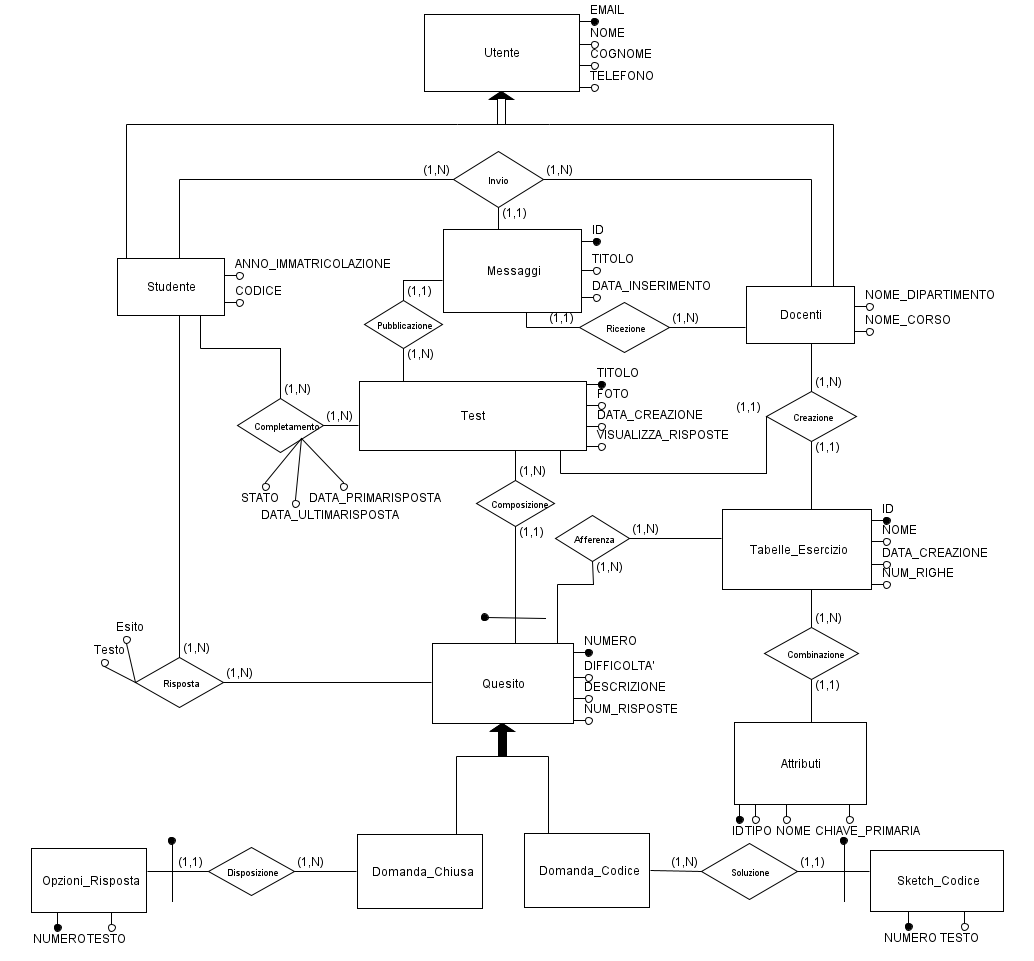
\includegraphics[width=0.7\textwidth]{foto1.png}
    \caption{Modello E-R precedente al raffinamento.}
\end{figure}

\subsection{Dizionario delle entità}
\begin{table}[H]
    \centering
    \begin{tabular}{|p{3.25cm}|p{4cm}|p{4cm}|p{3.75cm}|}
        \hline
        \bf Entità & \bf Descrizione & \bf Attributi & \bf Identificatore \\
        \hline
        Utente & Utilizzatore generale dell'applicativo & Email, Password, Nome, Cognome, Telefono & Email \\        
        \hline
        Studente & Studente  fruitore della piattaforma per la risoluzione dei quesiti posti & Email\_Studente, Anno\_Immatricolazione, Codice & Email\_Studente \\
        \hline
        Docente & Docente creatore e ideatore di quesiti e tabelle di esercizio & Email\_Docente, Nome\_Dipartimento, Nome\_Corso & Email\_Docente \\
        \hline
        Tabella\_Esercizio & Tabelle contenenti i meta-dati per la realizzazione di eventuali quesiti & Id, Email\_Docente, Nome, Data\_Creazione, Num\_Righe & Id \\
        \hline
        Attributo & Attributi parte costituente delle tabelle di esercizio, finalizzati per la realizzazione di quesiti & Id, Id\_Tabella, Tipo, Nome, Chiave\_Primaria & Id \\
        \hline
        Test & Test indica l'insieme di quesiti svolti dagli studenti e creati dal docente & Titolo, Email\_Docente, Foto, Data\_Creazione, Visualizza\_Risposte & Titolo \\
        \hline
        Quesito & Quesito relativo a tematiche svolte durante il corso & Id, Titolo\_Test, Difficoltà, Num\_Risposte, Descrizione & Id, Titolo\_Test \\
        \hline
        Domanda\_Chiusa & Tipologia di quesito, rappresentante una domanda a scelta multipla & Id\_Domanda\_Chiusa, Titolo\_Test & Id\_Domanda\_Chiusa, Titolo\_Test \\
        \hline
        Opzione\_Risposta & Opzioni di risposta relative ad una domanda chiusa & Id, Id\_Domanda\_Chiusa, Titolo\_Test, Testo, Soluzione & Id, Id\_Domanda\_Chiusa, Titolo\_Test \\
        \hline
        Domanda\_Codice & Tipologia di quesito, richiedente la formulazione di query SQL & Id\_Domanda\_Codice, Titolo\_Test & Id\_Domanda\_Codice, Titolo\_Test \\
        \hline
        Skecth\_Codice & Skecth di codice SQL risulutivi rispetto al quesito somministrato & Id, Id\_Domanda\_Codice, Titolo\_Test, Testo, Soluzione & Id, Id\_Domanda\_Codice, Titolo\_Test \\
        \hline
        Messaggio & Comunicazione inviata dal docente a tutti gli studenti & Id, Email\_Docente, Titolo\_Test, Testo, Titolo, Data\_Inserimento & Id \\
        \hline
        Messaggio\_Studente & Messaggio inviato dallo studente al docente del corso & Id\_Messaggio\_Studente, Email\_Studente & Id\_Messaggio\_Studente \\
        \hline
    \end{tabular}
    \caption{Descrizione dell'entità del modello E-R.}
\end{table}

\subsection{Dizionario delle relazioni}
\large
\begin{table}[H]
    \centering
    \begin{tabularx}{\textwidth}{|p{2.75cm}|p{4.25cm}|p{3cm}|p{4.75cm}|}
        \hline
        \bf Relazione & \bf Descrizione & \bf Componenti & \bf Attributi \\
        \hline
        Creazione & Creazione da parte di docenti di tabelle di esercizio e di test & Docente, Tabella\_Esercizio, Test & . \\
        \hline
        Completamento & Completamento di un test somministrato da parte degli studenti & Studente, Test & Email\_Studente, Titolo\_Test, Stato, Data\_Ultima\_Risposta, Data\_Prima\_Risposta \\
        \hline
        Invio & Invio di messaggi da parte di studenti & Studente, Messaggio\_Studente & . \\
        \hline
        Ricezione & Invio e ricezione di comunicazioni dal docente del corso & Docente, Messaggio & . \\
        \hline 
        Pubblicazione & Pubblicazione di comunicazioni afferenti ad uno specifico test & Messaggio, Test & . \\
        \hline
        Risposta & Risposta formulata dagli studenti in relazione ad uno specifico quesito & Studente, Quesito & Email\_Studente, Id\_Quesito, Titolo\_Test, Testo, Esito \\
        \hline
        Composizione & Composizione di un insieme di quesiti rispetto ad un determinato test & Quesito, Test & . \\
        \hline
        Afferenza & Afferenza dei quesiti ideati relativamente a tabelle di esercizio & Quesito, Tabella\_Esercizio & . \\
        \hline
        Combinazione & Combinazione di attributi per la costruzione di tabelle di esercizio & Attributo, Tabella\_Esercizio & . \\
        \hline
        Vincolo Integrità & Vincolo di integrità che mantiene tutti i vincoli referenziali tra attributi di tabelle di esercizio & Attributo & Referente, Referenziato\\
        \hline
        Disposizione & Disposizione del numero complessivo di opzioni di risposta relative alla domanda chiusa sottoposta & Opzione\_Risposta, Domanda\_Chiusa & . \\    
        \hline
        Soluzione & Soluzione insieme delle query SQL che risolvono la domanda di codice & Sketch\_Codice, Domanda\_Codice & . \\
        \hline
    \end{tabularx}
    \caption{Descrizione delle relazioni del modello E-R.}
\end{table}

\subsection{Tavola delle business rules}
\large
\begin{table}[h]
    \centering
    \begin{tabular}[center]{|p{13cm}|}
        \hline
        \bf Regole di vincolo \\
        \hline
        Il campo Codice alfanumerico degli studenti deve avere una lunghezza pari a 16 caratteri \\
        \hline
        Il docente può inserire i vincoli di integrità referenziale tra gli attributi che compongano tabelle di esercizio \\
        \hline
        Il numero progressivo associato ad un quesito è univoco, ma solo all'interno di uno specifico test \\
        \hline
        Il numero delle opzioni di risposta, sia per Domande\_Chiuse che per Domande\_Codice, è univoco, ma solo all'interno dello specifico quesito \\
        \hline
        Uno studente può sottomettere più risposte per lo stesso quesito, ma solo se il test non è in stato Concluso \\ 
        \hline 
        Un messaggio inviato da un docente è recapitato da tutti gli studenti del corso, invece un messaggio comunicato da uno studente è ricevuto dallo specifico docente \\
        \hline
        \bf Regole di derivazione \\ 
        \hline
        Il livello di difficoltà di ogni test consiste in un campo enum, che può assumere esclusivamente tre valori: Basso, Medio oppure Difficile \\
        \hline
        Il campo Num\_Risposte nell'entità Quesito è una ridondanza concettuale \\
        \hline 
        L'attributo Visualizza\_Risposte è un campo booleano, permette di visualizzare o meno le risposte dei quesiti \\
        \hline
        I campi Data\_PrimaRisposta e Data\_UltimaRisposta, della relazione Completamento, devono essere espressi su scala temporale \\
        \hline
        L'attributo della relazione Completamento è un campo enum, il quale può assumere esclusivamente tre valori: Aperto, InCompletamento e Concluso \\
        \hline 
        Il campo Esito della relazione Risposta è un attributo booleano, definisce la correttezza della risposta sottomessa \\
        \hline    
\end{tabular}
    \caption{Descrizione delle regole di vincolo e di derivazione non attuabili tramite il modello concettuale}
\end{table}

\newpage
\section{Progettazione logica}
\large
L'obiettivo di tale sezione promuove la realizzazione del modello logico a partire dalle informazioni del modello E-R. Tuttavia è bene attuare un insieme di possibili passaggi che possano favorire la traduzione, adeguando tematiche di efficienza e correttezza. Pertanto, come da capitolo seguente, è definita la ristrutturazione del diagramma E-R, affinchè sia agevolata la traduzione secondo il modello logico, ottimizzando il processo nella sua interezza.

\subsection{Modello E-R raffinato}
\large
\begin{figure}[H]
    \includegraphics*[width=0.75\textwidth]{foto2.png}
    \caption{Modello E-R successivo al raffinamento.}
\end{figure}

\subsection{Analisi delle ridondanze}
\large
In questa sezione sono riportate tutte le considerazioni necessarie per comprendere al meglio l'impatto delle ridondanze sullo schema E-R ideato; con conseguente definizione del costo operazionale sui dati di riferimento. Una fase simile è cruciale per stabilire se determinate informazioni comportano svantaggi significativi, come ad esempio maggiore occupazione di memoria oppure maggiore complessità degli aggiornamenti.\vspace{7pt}\\
Si definiscono le seguenti annotazioni:
\begin{itemize}[label={-}]
    \itemsep0em
    \item \textit{S$_r$}, lo schema E-R \textbf{con ridondanza}
    \item \textit{S}, \hspace{1px} lo schema E-R \textbf{senza ridondanza}
\end{itemize}
\vspace*{7pt}
Sono specificate un totale di quattro operazioni, relative al campo \textit{Num\_Risposte} dell'entità \textit{Quesito}, le quali si contraddistinguono in: \vspace*{7pt}\\
\hspace*{5pt}\textbf{OP1} \\
\hspace*{5pt}Aggiungere una nuova risposta ad un quesito esistente (10 volte/mese, interattiva) \vspace*{7pt}\\
\hspace*{5pt}\textbf{OP2} \\
\hspace*{5pt}Rimuovere un quesito e tutte le risposte ottenute (2 volte/mese, batch) \vspace*{7pt}\\
\hspace*{5pt}\textbf{OP3} \\
\hspace*{5pt}Visualizzare tutti gli utenti presenti nella piattaforma (1 volte/mese, batch) \vspace*{7pt}\\
\hspace*{5pt}\textbf{OP4} \\
\hspace*{5pt}Contare il numero di risposte per ciascun quesito presente nella piattaforma (2 volte/mese, \hspace*{6pt}interattiva) \vspace*{7pt}\\
Successivamente si calcolano i costi operazionali dello schema E-R con ridondanza, esplicitando tutti gli elementi necessari, suddivisi in:
\begin{itemize}[label={ }]
    \itemsep0em 
    \item {\small\textbf{TAVOLA ACCESSI.} \\ 1 per RISPOSTA, 1 per QUESITO} \vspace*{2pt}\\ C(OP1) = 10 * 1 * (2 * 2 + 0) = 40 \vspace*{2pt} 
    \item {\small\textbf{TAVOLA ACCESSI.} \\ 10 per RISPOSTA, 1 per QUESITO, 1 per DOMANDA\_CHIUSA o 1 per DOMANDA\_CODICE} \vspace*{2pt}\\ C(OP2) = 2 * 0.5 * (2 * 12 + 0) = 24 \vspace*{2pt}
    \item {\small\textbf{TAVOLA ACCESSI.} \\ 50 per UTENTE, 50 per STUDENTE o 50 per DOCENTI} \vspace*{2pt}\\ C(OP3) = 1 * 0.5 * (0 + 100) = 50
    \item {\small\textbf{TAVOLA ACCESSI.} \\ 20 per QUESITO, 20 per DOMANDA\_CHIUSA o 20 DOMANDA\_CODICE } \vspace*{1pt}\\ C(OP4) = 2 * 1 * (0 + 40) = 80
\end{itemize}
\hspace*{15pt}C(S$_r$) = 40 + 24 + 50 + 80 = 194 \vspace*{7pt}\\
Si calcolano i costi operazionali dello schema E-R senza ridondanza, suddivisi in:
\begin{itemize}[label={ }]
    \itemsep0em 
    \item {\small\textbf{TAVOLA ACCESSI.} \\ 1 per RISPOSTA} \vspace*{2pt}\\ C(OP1) = 10 * 1 * (2 * 1 + 0) = 20 \vspace*{2pt} 
    \item {\small\textbf{TAVOLA ACCESSI.} \\ 10 per RISPOSTA, 1 per QUESITO, 1 per DOMANDA\_CHIUSA o 1 per DOMANDA\_CODICE} \vspace*{2pt}\\ C(OP2) = 2 * 0.5 * (2 * 12 + 0) = 24 \vspace*{2pt}
    \item {\small\textbf{TAVOLA ACCESSI.} \\ 50 per UTENTE, 50 per STUDENTE o 50 per DOCENTI} \vspace*{2pt}\\ C(OP3) = 1 * 0.5 * (0 + 100) = 50
    \item {\small\textbf{TAVOLA ACCESSI.} \\ 200 per RISPOSTA, 20 per QUESITO, 20 per DOMANDA\_CHIUSA o 20 per DOMANDA\_CODICE} \vspace*{2pt}\\ C(OP4) = 2 * 1 * (0 + 240) = 480
\end{itemize}
\hspace*{15pt}C(S) = 20 + 24 + 50 + 480 = 564 \vspace*{7pt} \vspace*{7pt}\\
Si osserva ora l'occupazione di memoria di entrambi i diagrammi, in cui si manifesta:
\begin{itemize}[label={-}]
    \itemsep0em
    \item M(S$_r$) = X + 20 * 4 = X + 80 byte
    \item M(S) = \hspace*{1pt}X byte
\end{itemize}
Terminate tutte le operazioni riferite all'analisi delle ridondanze, si osserva come il mantenimento comporti a vantaggi significativi, piuttosto che l'eliminazione. Infatti il rapporto $C(S) \div C(S_r)$ restituisce un valore che si aggira attorno a 3, in questo caso è conveniente mantenere l'attributo \textit{Num\_Risposte}, dettata anche dall'irrisorio overhead introdotto, pari a 80 byte.

\subsection{Lista delle tabelle con i vincoli di chiave}
\large
Dopo aver svolto le fasi principali che agevolano il processo di traduzione, nella sezione consecutiva si osserva la descrizione del modello logico di riferimento, il quale fornisce l'insieme di tabelle che caratterizzano il database e i differenti attributi relativi ad ogni specifica relazione. Si evidenzia la presenza delle chiavi primarie, segnalate attraverso una sottolineatura delle colonne che compongano il vincolo.\vspace*{7pt}
\begin{itemize}[label={ }, leftmargin=*, wide=1pt]
    \itemsep0em
    \item Utente(\underline{EMAIL}, PASSWORD, NOME, COGNOME, TELEFONO)
    \item Studente(\underline{EMAIL\_STUDENTE}, ANNO\_IMMATRICOLAZIONE, CODICE)
    \item Docente(\underline{EMAIL\_DOCENTE}, NOME\_DIPARTIMENTO, NOME\_CORSO)
    \item Tabella\_Esercizio(\underline{ID}, EMAIL\_DOCENTE, NOME, DATA\_CREAZIONE, NUM\_RIGHE)
    \item Attributo(\underline{ID}, ID\_TABELLA, TIPO, NOME, CHIAVE\_PRIMARIA)
    \item Vincolo\_integrita(\underline{REFERENTE}, \underline{REFERENZIATO})
    \item Test(\underline{TITOLO}, EMAIL\_DOCENTE, FOTO, DATA\_CREAZIONE, VISUALIZZA\_RISPOSTA)
    \item Quesito(\underline{ID}, \underline{TITOLO\_TEST}, DIFFICOLTA, NUM\_RISPOSTE, DESCRIZIONE)
    \item Afferenza(\underline{ID\_QUESITO}, \underline{TITOLO\_TEST}, \underline{ID\_TABELLA})
    \item Domanda\_Chiusa(\underline{ID\_DOMANDA\_CHIUSA}, \underline{TITOLO\_TEST})
    \item Opzione\_Risposta(\underline{ID}, \underline{ID\_DOMANDA\_CHIUSA}, \underline{TITOLO\_TEST}, TESTO, SOLUZIONE)
    \item Domanda\_Codice(\underline{ID\_DOMANDA\_CODICE}, \underline{TITOLO\_TEST})
    \item Skecth\_Codice(\underline{ID}, \underline{ID\_DOMANDA\_CODICE}, \underline{TITOLO\_TEST}, TESTO, SOLUZIONE)
    \item Completamento(\underline{TITOLO\_TEST}, \underline{EMAIL\_STUDENTE}, STATO, DATA\_ULTIMA\_RISPOSTA, DATA\_PRIMA\_RISPOSTA)
    \item Risposta(\underline{EMAIL\_STUDENTE}, \underline{ID\_QUESITO}, \underline{TITOLO\_TEST}, TESTO, ESITO)
    \item Messaggio(\underline{ID}, EMAIL\_DOCENTE, TITOLO\_TEST, TESTO, TITOLO, DATA\_INSERIMENTO)
    \item Messaggio\_Studente(\underline{ID\_MESSAGGIO\_STUDENTE}, EMAIL\_STUDENTE)
\end{itemize}

\subsection{Lista dei vincoli inter-relazionali}
\large
Quest'ultima parte del capitolo, riporta in maniera esplicita tutti i vincoli inter-relazionali che intercorrono tra le differenti tabelle, disposti nello stesso ordine in cui sono visualizzate le relazioni nel paragrafo precedente.
\begin{itemize}[label={ }, leftmargin=*, wide=1pt]
    \itemsep0em
    \item Studente.EMAIL\_STUDENTE \textbf{-->} Utente.EMAIL
    \item Docente.EMAIL\_DOCENTE \textbf{-->} Utente.EMAIL
    \item Tabella\_Esercizio.EMAIL\_DOCENTE \textbf{-->} Docente.EMAIL\_DOCENTE
    \item Attributo.ID\_TABELLA \textbf{-->} Tabella\_Esercizio.ID
    \item Vincolo\_Integrità.REFERENTE \textbf{-->} Attributo.ID
    \item Vincolo\_Integrità.REFERENZIATO \textbf{-->} Attributo.ID
    \item Test.EMAIL\_DOCENTE \textbf{-->} Docente.EMAIL\_DOCENTE
    \item Quesito.TITOLO\_TEST \textbf{-->} Test.TITOLO
    \item Afferenza.ID\_QUESITO \textbf{-->} Quesito.ID
    \item Afferenza.TITOLO\_TEST \textbf{-->} Quesito.TITOLO\_TEST
    \item Afferenza.ID\_TABELLA \textbf{-->} Tabella\_Esercizio.ID
    \item Domanda\_Chiusa.ID\_DOMANDA\_CHIUSA \textbf{-->} Quesito.ID
    \item Domanda\_Chiusa.TITOLO\_TEST \textbf{-->} Quesito.TITOLO\_TEST
    \item Opzione\_Risposta.ID\_DOMANDA\_CHIUSA \textbf{-->} Domanda\_Chiusa.ID\_DOMANDA\_CHIUSA 
    \item Opzione\_Risposta.TITOLO\_TEST \textbf{-->} Domanda\_Chiusa.TITOLO\_TEST 
    \item Domanda\_Codice.ID\_DOMANDA\_CODICE \textbf{-->} Quesito.ID
    \item Domanda\_Codice.TITOLO\_TEST \textbf{-->} Quesito.TITOLO\_TEST
    \item Skecth\_Codice.ID\_DOMANDA\_CODICE \textbf{-->} Domanda\_Codice.ID\_DOMANDA\_CODICE
    \item Skecth\_Codice.TITOLO\_TEST \textbf{-->} Domanda\_Codice.TITOLO\_TEST
    \item Completamento.EMAIL\_STUDENTE \textbf{-->} Studente.EMAIL\_STUDENTE
    \item Completamento.TITOLO\_TEST \textbf{-->} Test.TITOLO
    \item Risposta.EMAIL\_STUDENTE \textbf{-->} Studente.EMAIL\_STUDENTE
    \item Risposta.ID\_QUESITO \textbf{-->} Quesito.ID
    \item Risposta.TITOLO\_TEST \textbf{-->} Quesito.TITOLO\_TEST
    \item Messaggio.EMAIL\_DOCENTE \textbf{-->} Docente.EMAIL\_DOCENTE
    \item Messaggio.TITOLO\_TEST \textbf{-->} Test.TITOLO
    \item Messaggio\_Studente.ID\_MESSAGGIO\_STUDENTE \textbf{-->} Messaggio.ID
    \item Messaggio\_Studente.TITOLO\_TEST \textbf{-->} Studente.EMAIL\_STUDENTE
\end{itemize}
       
\section{Descrizione delle funzionalità}
\large
\textbf{Registrazione}\\
Studenti e docenti hanno l'opportunità di registrarsi alla piattaforma, affinchè possano usufruire delle funzionalità implementate.\vspace*{7pt}\\
\textbf{Accedi}\\
Nuovamente, studenti e docenti, dopo essersi registrati, devono accedere alla piattaforma pur di poter utilizzare le funzionalità implementate.\vspace*{7pt}\\
\textbf{Logout}\\
L'utente qualora abbia terminato di utilizzare la piattaforma, detiene la possibilità di disconnetersi, visualizzando la schermata home.\vspace*{7pt}\\
\textbf{Creazione}\\
In relazione alla funzionalità proposta, occorre suddividere le azioni che uno studente oppure un docente potrebbe eseguire. Pertanto di seguito è definita una breve suddivisione, in cui: 
\begin{itemize}[label={-}]
    \itemsep0em
    \item Docente, effettuato l'accesso può creare una nuova tabella, un nuovo test, un nuovo quesito ed infine inviare messaggi a tutti gli studenti
    \item Studente, effettuato l'accesso può inviare messaggi allo specifico docente titolare del test
\end{itemize}    
\textbf{Eliminazione}\\
L'eliminazione riguarda solo la figura del docente, pertanto esso è in grado di eliminare una tabella, se non possiede vincoli di integrità referenziale, un quesito e un test.\vspace*{7pt}\\
\textbf{Svolgi test}\\
In questo caso si tratta di una funzionalità circoscritta agli studenti, per cui, visualizzando i test disponibili, uno studente ha la possibilità di svolgere un tentativo risolutivo del test di riferimento; ciò può avvennire più volte anche per lo stesso test.\vspace*{7pt}\\
\textbf{Visualizza}\\
Come avviene per la creazione, occorre distinguere le azioni che possano essere conseguite a seconda della tipologia dell'utente, suddivise in:
\begin{itemize}[label={-}]
    \itemsep0em
    \item Docente, può visualizzare le specifiche di una tabella, di un quesito, di un test, dei messaggi inviati e ricevuti
    \item Studente, può visualizzare le risposte, le soluzioni e il file multimediale connessi ad un test, i messaggi inviati e ricevuti
\end{itemize}

\newpage
\section{SQL}
\begin{lstlisting}[language=SQL, title=Codice SQL completo dello schema della base di dati.]
DROP DATABASE IF EXISTS ESQLDB;
CREATE DATABASE IF NOT EXISTS ESQLDB;

USE ESQLDB;

CREATE TABLE Utente(
    EMAIL VARCHAR(255) PRIMARY KEY,
    PSWD VARCHAR(255),
    NOME VARCHAR(255) NOT NULL,
    COGNOME VARCHAR(255) NOT NULL,
    TELEFONO INT(10)
)ENGINE=INNODB ;

CREATE TABLE Studente(
    EMAIL_STUDENTE VARCHAR(255) PRIMARY KEY,
    ANNO_IMMATRICOLAZIONE INT(4) NOT NULL,
    CODICE VARCHAR(16) NOT NULL,
    FOREIGN KEY (EMAIL_STUDENTE) REFERENCES Utente(EMAIL) ON DELETE CASCADE
)ENGINE=INNODB ;

CREATE TABLE Docente(
    EMAIL_DOCENTE VARCHAR(255) PRIMARY KEY,
    NOME_DIPARTIMENTO VARCHAR(255) NOT NULL,
    NOME_CORSO VARCHAR(255) NOT NULL,
    FOREIGN KEY (EMAIL_DOCENTE) REFERENCES Utente(EMAIL) ON DELETE CASCADE
)ENGINE=INNODB ;

CREATE TABLE Tabella_Esercizio(
    ID INT AUTO_INCREMENT PRIMARY KEY,
    NOME VARCHAR(255) NOT NULL,
    DATA_CREAZIONE DATETIME NOT NULL,
    NUM_RIGHE INT NOT NULL,
    EMAIL_DOCENTE VARCHAR(255) NOT NULL,
    FOREIGN KEY(EMAIL_DOCENTE) REFERENCES Docente(EMAIL_DOCENTE) ON DELETE CASCADE
)ENGINE=INNODB ;

CREATE TABLE Attributo(
    ID INT AUTO_INCREMENT PRIMARY KEY,
    ID_TABELLA INT,
    TIPO VARCHAR(255) NOT NULL,
    NOME VARCHAR(255) NOT NULL,
    CHIAVE_PRIMARIA BOOLEAN NOT NULL,
    FOREIGN KEY(ID_TABELLA) REFERENCES Tabella_Esercizio(ID) ON DELETE CASCADE 
)ENGINE=INNODB ;

CREATE TABLE Vincolo_Integrita(
    REFERENTE INT,
    REFERENZIATO INT,
    PRIMARY KEY(REFERENTE, REFERENZIATO),
    FOREIGN KEY(REFERENTE) REFERENCES Attributo(ID) ON DELETE CASCADE,
    FOREIGN KEY(REFERENZIATO) REFERENCES Attributo(ID) ON DELETE CASCADE
)ENGINE=INNODB ;

CREATE TABLE Test(
    TITOLO VARCHAR(255) PRIMARY KEY,
    EMAIL_DOCENTE VARCHAR(255) NOT NULL,
    FOTO LONGBLOB,
    DATA_CREAZIONE DATE NOT NULL,
    VISUALIZZA_RISPOSTE BOOLEAN NOT NULL,
    FOREIGN KEY (EMAIL_DOCENTE) REFERENCES Docente(EMAIL_DOCENTE) ON DELETE CASCADE
)ENGINE=INNODB ;

CREATE TABLE Quesito(
    ID INT,
    TITOLO_TEST VARCHAR(255),
    DIFFICOLTA ENUM('BASSO', 'MEDIO', 'ALTO') NOT NULL,
    NUM_RISPOSTE INT NOT NULL,
    DESCRIZIONE VARCHAR(255) NOT NULL,
    PRIMARY KEY(ID, TITOLO_TEST),
    FOREIGN KEY(TITOLO_TEST) REFERENCES Test(TITOLO) ON DELETE CASCADE
)ENGINE=INNODB ;

CREATE TABLE Afferenza(
    ID_QUESITO INT,
    TITOLO_TEST VARCHAR(255),
    ID_TABELLA INT,
    PRIMARY KEY(ID_QUESITO, TITOLO_TEST, ID_TABELLA),
    FOREIGN KEY(ID_QUESITO, TITOLO_TEST) REFERENCES Quesito(ID, TITOLO_TEST) ON DELETE CASCADE,
    FOREIGN KEY(ID_TABELLA) REFERENCES Tabella_Esercizio(ID) ON DELETE CASCADE
)ENGINE=INNODB ;

CREATE TABLE Domanda_Chiusa(
    ID_DOMANDA_CHIUSA INT,
    TITOLO_TEST VARCHAR(255),
    PRIMARY KEY (ID_DOMANDA_CHIUSA, TITOLO_TEST),
    FOREIGN KEY(ID_DOMANDA_CHIUSA, TITOLO_TEST) REFERENCES Quesito(ID, TITOLO_TEST) ON DELETE CASCADE 
)ENGINE=INNODB ;

CREATE TABLE Opzione_Risposta(
    ID INT,
    ID_DOMANDA_CHIUSA INT,
    TITOLO_TEST VARCHAR(255),
    TESTO TEXT NOT NULL,
    SOLUZIONE BOOLEAN NOT NULL,
    PRIMARY KEY(ID, ID_DOMANDA_CHIUSA, TITOLO_TEST),
    FOREIGN KEY(ID_DOMANDA_CHIUSA, TITOLO_TEST) REFERENCES Domanda_Chiusa(ID_DOMANDA_CHIUSA, TITOLO_TEST) ON DELETE CASCADE    
)ENGINE=INNODB ;

CREATE TABLE Domanda_Codice(
    ID_DOMANDA_CODICE INT,
    TITOLO_TEST VARCHAR(255),
    PRIMARY KEY(ID_DOMANDA_CODICE, TITOLO_TEST),
    FOREIGN KEY(ID_DOMANDA_CODICE, TITOLO_TEST) REFERENCES Quesito(ID, TITOLO_TEST) ON DELETE CASCADE    
)ENGINE=INNODB ;

CREATE TABLE Sketch_Codice(
    ID INT,
    ID_DOMANDA_CODICE INT,
    TITOLO_TEST VARCHAR(255),
    TESTO TEXT NOT NULL,
    SOLUZIONE BOOLEAN NOT NULL,
    PRIMARY KEY(ID, ID_DOMANDA_CODICE, TITOLO_TEST),
    FOREIGN KEY(ID_DOMANDA_CODICE, TITOLO_TEST) REFERENCES Domanda_Codice(ID_DOMANDA_CODICE, TITOLO_TEST) ON DELETE CASCADE    
)ENGINE=INNODB ;

CREATE TABLE Completamento(
    TITOLO_TEST VARCHAR(255), 
    EMAIL_STUDENTE VARCHAR(255),
    STATO ENUM('APERTO', 'INCOMPLETAMENTO', 'CONCLUSO') NOT NULL, 
    DATA_ULTIMARISPOSTA DATETIME,
    DATA_PRIMARISPOSTA DATETIME,
    PRIMARY KEY(TITOLO_TEST, EMAIL_STUDENTE),
    FOREIGN KEY(TITOLO_TEST) REFERENCES Test(TITOLO) ON DELETE CASCADE,
    FOREIGN KEY(EMAIL_STUDENTE) REFERENCES Studente(EMAIL_STUDENTE) ON DELETE CASCADE
)ENGINE=INNODB ;

CREATE TABLE Risposta(
    EMAIL_STUDENTE VARCHAR(255),
    ID_QUESITO INT,
    TITOLO_TEST VARCHAR(255),
    TESTO TEXT NOT NULL,
    ESITO BOOLEAN NOT NULL,
    PRIMARY KEY(EMAIL_STUDENTE, ID_QUESITO, TITOLO_TEST),
    FOREIGN KEY(EMAIL_STUDENTE) REFERENCES Studente(EMAIL_STUDENTE) ON DELETE CASCADE,
    FOREIGN KEY(ID_QUESITO, TITOLO_TEST) REFERENCES Quesito(ID, TITOLO_TEST) ON DELETE CASCADE
)ENGINE=INNODB ;

CREATE TABLE Messaggio(
    ID INT AUTO_INCREMENT PRIMARY KEY,
    EMAIL_DOCENTE VARCHAR(255) NOT NULL,
    TESTO TEXT NOT NULL,
    TITOLO VARCHAR(255) NOT NULL,
    TITOLO_TEST VARCHAR(255) NOT NULL,
    DATA_INSERIMENTO DATE NOT NULL,
    FOREIGN KEY(TITOLO_TEST) REFERENCES Test(TITOLO) ON DELETE CASCADE,
    FOREIGN KEY(EMAIL_DOCENTE) REFERENCES Docente(EMAIL_DOCENTE) ON DELETE CASCADE
)ENGINE=INNODB ;

CREATE TABLE Messaggio_Studente(
    ID_MESSAGGIO_STUDENTE INT PRIMARY KEY,
    EMAIL_STUDENTE VARCHAR(255) NOT NULL,
    FOREIGN KEY(ID_MESSAGGIO_STUDENTE) REFERENCES Messaggio(ID) ON DELETE CASCADE,
    FOREIGN KEY(EMAIL_STUDENTE) REFERENCES Studente(EMAIL_STUDENTE) ON DELETE CASCADE
)ENGINE=INNODB ;
\end{lstlisting}

\end{document}